\chapter{Fiber-optic sensing}\label{txt.sensing}

Light has revolutionized data transmission and made high data rates possible using optical fibers and laser diodes. Apart from the intended usage, data transmission lines made from optical fibers have a new use case in sensing. The optical fiber can be used to measure useful external properties thanks to the detection and analysis of different light scattering effects of the interaction between the light and the fiber, as discussed in Section~\ref{txt.scattering}.

This chapter will discuss fiber optics, optical reflectometry, distributed sensing, and different light scattering effects in the fiber.




\section{Fiber optic sensors}

Fiber optic sensors have three main parts - a \textit{light source}, a \textit{medium} that light passes through, and a \textit{detector}. The principle these sensors use is to generate light at the \textit{source} light (laser diode LD), then passes through the medium, which can be a scanned material or an optical fiber (Section~\ref{txt.optical.fibers}). The medium affects the light signal and changes signal properties measured at the detector. This way, fiber optic sensors can detect external properties such as vibrations (seismic, acoustic), pressure, acceleration, rotation, and chemical properties.

There are two types of sensors based on the medium used\footnote{https://www.rp-photonics.com/fiber\_optic\_sensors.html}:
\begin{itemize}
    \item \textit{intrinsic sensors} - the optical fiber is a measuring medium.
    \item \textit{extrinsic sensors} - use optical fiber to get the signal to and from the actual sensor.
\end{itemize}

There are two types of optical fiber sensors based on the location of the measurement:
\begin{enumerate}
    \item \textbf{Point} - These sensors measure only at the location of the transducer\footnote{device transforming energy from one form of energy to another form of energy}
    \item \textbf{Quasi-distributed} - They use many sensors along the fiber to measure 
    \item \textbf{Distributed} - The sensing element is the optical wire. It can measure at thousands of points along the optical wire thanks to different scattering effects, as discussed in Section~\ref{txt.scattering}. It can use existing telecommunication infrastructure to build the sensing network.
\end{enumerate}

\subsection{Fiber-optic sensing applications in different fields}\label{txt.sensing.usage}

The advantage of fiber optic sensing compared to other kinds of sensing is that it is immune to signal interference. The optic fiber is made of glass or transparent plastic. It can be used in environments that would be dangerous or harsh for other types of sensors. It is good to mention environments such as flammable, explosive, harsh chemicals, high voltage, or environments that would create electromagnetic noise. Thanks to these properties, fiber-optic sensing has many different applications.

The applications include:

\begin{itemize}
    \item \textit{Fiber-optic gyroscopes} - rotation measurement thanks to the Sagnac effect. They can replace older ring-laser technology~\cite{fog}.
    \item \textit{Fiber-optic accelerometers} - vibration measurements with added electromagnetic interference immunity~\cite{accelerometer}. 
    \item \textit{Fiber-optic bio-sensors} - thanks to glass fibers' chemical and thermal stability, these sensors are perfect for measuring harsh chemicals. Measurements can be done in hard-to-get or small spaces. They also measure on small sample volumes~\cite{chemsens}.
    \item \textit{Vibration detection} - seismic, acoustic,  and even underwater.
    \begin{itemize}
        \item \texttt{Seismology} - measuring and locating earthquakes~\cite{dasKislov}.
        \item \texttt{Building monitoring} - bridge monitoring for changes such as cracks~\cite{DVSShanFu}.
        \item \texttt{Perimeter protection} - detecting and localizing intrusion into an area, more in Section~\ref{txt.perimeter.security}.
        \item \texttt{Location detection} - fiber-optic sensors can detect traffic and vehicles in cities and on highways or locate trains along train tracks~\cite{dasKislov}.
        \item \texttt{Fiber-optic hydrophones} - under-water detection systems for seismic monitoring~\cite{hydrophones}.
    \end{itemize}
\end{itemize}

\subsection{Perimeter security}\label{txt.perimeter.security}

In the early 2000s, perimeter protection using fiber optics was based on breaking or cutting the fiber, triggering an alarm. This is good enough for one-time use because after the wire is broken, there is no choice but to replace or repair the wire. This system can not tell the location when using a single wire. Newer systems used \textit{Sagnac effect}, which uses a Sagnac interferometer and a closed loop made of fiber optic wires, for example, 3x3\footnote{three by three} wire system. Sagnac interferometer detects changes in the phase of light, and thanks to signal processing and calculating the time difference between amplitudes, the position of an intruder is calculated. Such an interferometer has a conversion unit from optical to electric signal. The electric signal is then sampled using a fast A/D converter with high sampling rates. The accuracy of such a system is 20-50 meters which is more than sufficient for perimeter protection~\cite{perimeterpolsko}. 

\begin{figure}
    \centering
    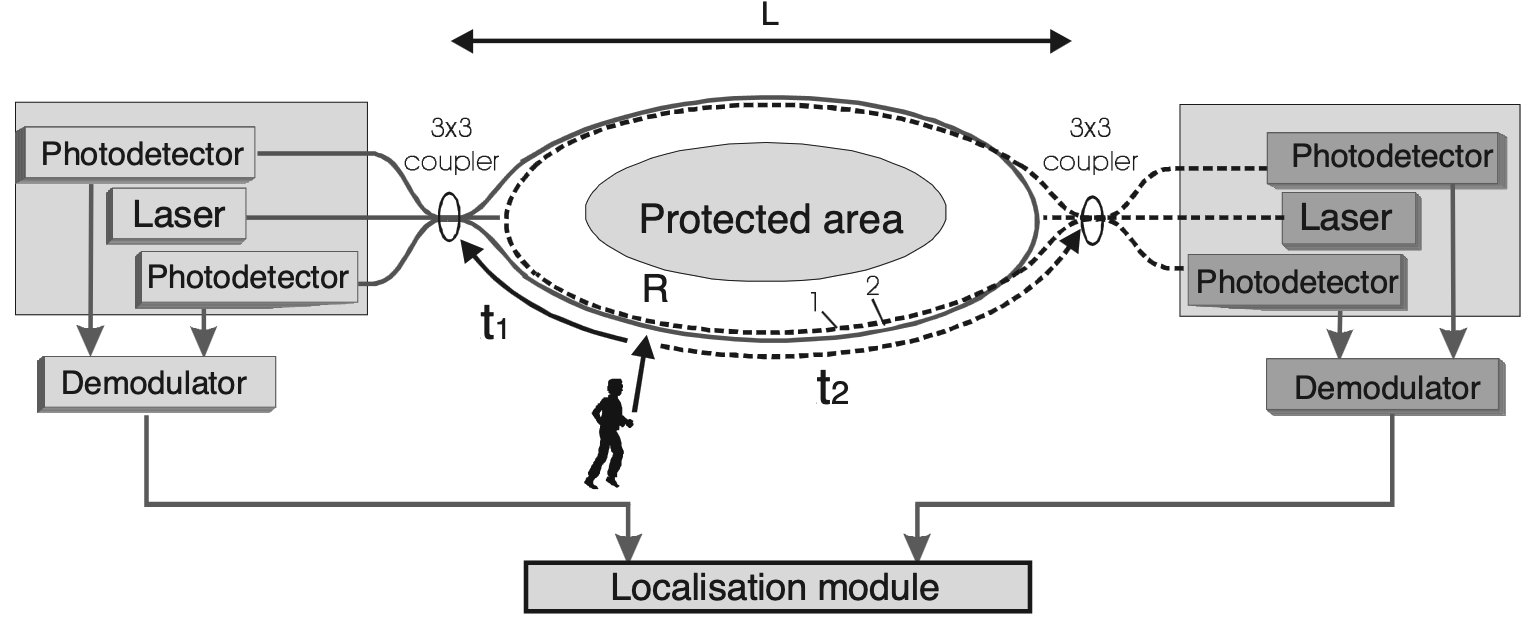
\includegraphics[width=\linewidth]{obrazky/sagnac_interrogator.png}
    \caption{3x3 system for perimeter protection using two Sagnac interferometers~\cite{perimeterpolsko}.}
    \label{fig:sagnac}
\end{figure}

Thanks to research and technological advancements, new devices based on \ac{das} systems are used. These systems use scattering effects that happen in the fiber during the passage of photons through the fiber's medium. These effects are then analyzed at the source of light. The light bounces from imperfections in the fiber and is propagated backward as scattering (\textit{backs-cattering}). Nothing special happens when the fiber is not moving, but when the fiber is affected in any way, for example, by vibrations of an intruder or just by voice alone, the back-scattering changes. These changes can then be analyzed and categorized as an intrusion.


\section{Optical fibers}\label{txt.optical.fibers}


As optical sensing uses existing fiber optic transmission lines, it is important to account for different kinds of optical fibers, materials, and production methods. Optical fibers consist of three main elements \textit{core}, \textit{cladding}, and \textit{coating}. Materials from which core and cladding are made are plastic or glass $Si_2O_3$. 

All-glass fiber dopants, such as $GeO_2$, $P_2O_5$, $B_2O_3$, can be added to all-glass fibers to adjust the refractive index. The core usually has a higher refractive index than cladding by about \qty{1}{\si{\percent}}. Lowering the refractive index can be done by doping fluorine, which is done in the core when the refracting index is too high and needs to be lowered\footnote{https://www.rp-photonics.com/fiber\_core.html}. The radius of core ranges from \qty{3.7}{\si{\micro}\meter} to \qty{200}{\micro\meter} and radius of cladding is up-to \qty{140}{\si{\micro}\meter}~\cite{cabling}.

Plastic optics uses organic material in the form of polymers - chains. Materials used are acrylic, polycarbonate, polystyrene, or liquid silicone. The core of plastic fiber has a popular diameter of \qty{980}{\si{\micro}\meter}.

Although the purpose of the coating is simply protection, the fiber would be very fragile without it. It is usually without special color but can be painted to ease the identification of individual fibers. There are multiple layers of coating, at least primary and secondary. The primary coating is softer to allow the bending of the fiber. Secondary is harder to protect inner layers. Materials such as acrylate, silicone, polyimide,e or carbon are used depending on the application of the optical fiber. for example. For example, acrylate has limited temperature resistance; in this case, silicone is better as it is heat resistant up to \qty{200}{\celsius}\cite{cabling}. For more extreme applications, Polyimide is used as it can withstand temperatures up to \qty{350}{\celsius}, and it is also resistant to chemicals and abrasion~\cite{cabling}.

% \subsection{Fiber modality}\label{txt.optical.fibers.modality}

% Optical fibers can have different kinds of modality depending on manufacturing processes and desired properties of the material. We differentiate multimode and single-mode fiber optic cables. 

% Multimode optical fibers have much larger core diameter compared to the diameter of cladding. This enables 
% %TODO


% Single mode fibers have single propagation mode  per polarization fir a given wavelength. They have very small core diameter, only few micrometers, relative to the cladding diameter. Since they use only single mode there is no inter-modal dispersion\footnote{https://www.rp-photonics.com/single\_mode\_fibers.html}
% %TODO

\section{Light scattering effects in fiber optics}\label{txt.scattering}

Light precisely photons traveling through a medium - atmosphere, glasses, glass optical fiber, or any other medium can bounce from what is called \textit{scattering centers} in the medium. \textit{Scattering centers} are any non-uniformities in the medium such as vacancy defects (missing atoms in otherwise uniform structure), foreign particles, bubbles, trapped gas molecules, fractures, micro-cracks, any changes in refractive index, density fluctuations, manufacturing imperfections, and others~\cite{scatteringcenterbook}. Scattering centers create different kinds of scattering, as will be discussed in the next sections. They include \textit{Mie scattering} (Section~\ref{txt.scattering.mie}), \textit{Rayleigh scattering} (Section~\ref{txt.scattering.ray}), \textit{Raman scattering} (Section~\ref{txt.scattering.ram}) or \textit{Brillouin scattering} (Section~\ref{txt.scattering.bril}). For comparison, Figure~\ref{fig:scattering.comparison} shows all of these different scattering effects:

\begin{itemize}
    \item 1 - input radiation from a laser diode.
    \item 2 - Rayleigh scattering 
    \item 3 and 4 - Brillouin scattering lines %TODO stokes antistokes
    \item 5 and 6 - Raman scattering 
\end{itemize}

\begin{figure}
    \centering
    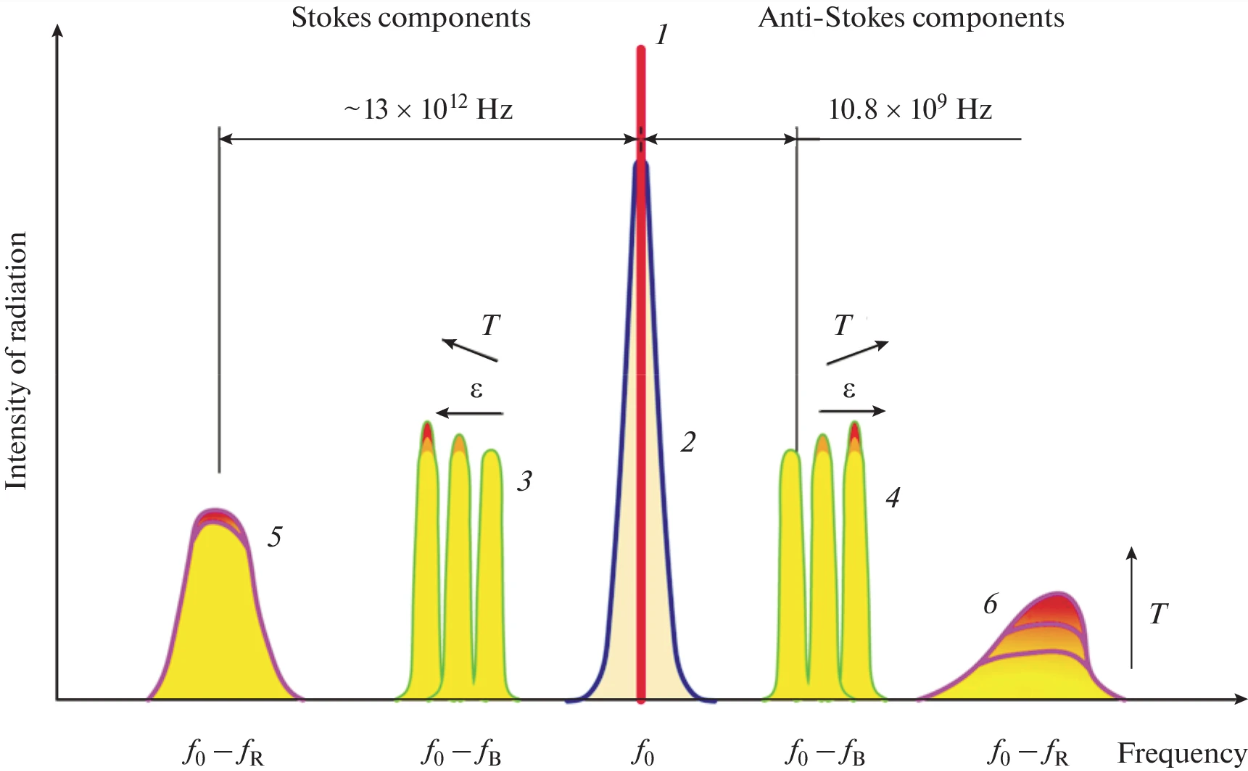
\includegraphics[width=\linewidth]{obrazky/scatterings.png}
    \caption{Comparison of different scattering effects~\cite{scattering.comparison}.}
    \label{fig:scattering.comparison}
\end{figure}

\subsection{Mie scattering}\label{txt.scattering.mie}

\textit{Mie scattering} is an optical phenomenon happening when light traveling through a medium bounces from \textit{scattering centers} the same length or bigger than the wavelength of the light. Mie scattering applies to any spherical particles located in the medium. This also applies to the smaller particles. But we distinguish Mie scattering for particles bigger than the wavelength of light for clarity. For particles smaller than the wavelength of light we distinguish a special case of Mie scattering, and we call it \textit{Rayleigh scattering}, which will be discussed in the next Section~\ref{txt.scattering.ray}. That said, there are differences between these two types. The scattered light's amplitudes are stronger for forward scattering in Mie scattering\footnote{https://www.rp-photonics.com/rayleigh\_scattering.html}. Large defects are usually not uniformly distributed along the fiber, which prevents it from being used in \ac{das} systems~\cite{dasKislov}.

\subsection{Rayleigh scattering}\label{txt.scattering.ray}

Rayleigh scattering is an optical phenomenon named after British physicist Lord Rayleigh. Light is scattered from scattering centers much smaller than the wavelength of the light, for example, individual molecules or atoms. This is opposite to Mie scattering \ref{txt.scattering.mie}, where light is scattering from larger scattering centers. The difference is that amplitudes are the same for forward and backscattering in Rayleigh scattering\footnote{https://www.rp-photonics.com/rayleigh\_scattering.html}. Compared to other scattering processes, Rayleigh is \textit{linear} scattering process whereas \textit{Raman} and \textit{Brillouin} scatterings are \textit{nonlinear}\footnote{Nonlinear light effects occur when the output intensity does not increase proportionally to the input intensity; for example doubling the optical input intensities does not result in double the output intensity. These nonlinear effects tend to weaken significantly at low optical intensities.}.

Only a small portion of the back-scattered light returns to the source - most of it leaves the fiber on the sides. Rayleigh scattering is used in \ac{das}, as discussed in Section~\ref{txt.das}.

When solidified in a medium, not all scattering centers cause Rayleigh scattering. At a wavelength of about 0.95 μm (microns), glass optical fibers have a high attenuation band caused by scattering and absorption by hydroxide ions~\cite{scatteringcenterbook}. Silica glass is an amorphous material with random density fluctuations due to its irregular microscopic structure. This can be limited by an annealing process but can not be removed completely\footnote{https://www.rp-photonics.com/rayleigh\_scattering.html}.




\subsection{Raman scattering}\label{txt.scattering.ram}

The effect photons have when interacting with the crystal lattice of glass is called \textit{Raman scattering}. A transparent optical medium, such as glass, has a crystal lattice. The lattice is naturally vibrating, causing a delayed nonlinear response to the light passing through it. The photon traveling through the medium experiences a loss in energy due to interactions with the medium. This is also called \textit{inelastic scattering}. This is further explained in the next Section~\ref{txt.scattering.bril}.

% The losses happen as vibration energy is exchanged between what are called \textit{phonos}. 

Raman scattering can be measured by sending two light waves with different wavelengths through the optical medium. The  signal with longer wavelength experiences optical amplification at the expense of the one with a shorter wavelength. This is used in Raman lasers, Raman amplifiers, or Raman spectroscopy\footnote{https://www.rp-photonics.com/raman\_scattering.html}.


\subsection{Brillouin scattering}\label{txt.scattering.bril}

Also known as \textit{Mandelsam-Brillouin scattering}, it was first described by Raman in the 1920s. Brillouin scattering is a scattering effect created when light traveling through a medium is scattered during interaction with thermal vibrations of these molecules. As described earlier, it is very similar to Raman scattering. The intensity is much lower than Rayleigh scattering; see Section~\ref{txt.scattering.ray}. But at the same time, much stronger than Raman scattering. For comparison, see Figure~\ref{fig:scattering.comparison}.

The difference between Raman and Brillouin scattering is in the type of interactions with vibrations of the crystal lattice and molecules. To describe the fundamental quanta of lattice vibrations involved in these interactions, we use the term \textit{phonons}. 

There are two types of phonons:

\begin{itemize}
    \item \textit{acoustic phonons} - associated with backward Brillouin scattering; show linear dispersion relation in bulk. 
    \item \textit{optical phonons} - associated with Raman scattering relate to molecular vibrations; have flat dispersion. The forward Brillouin scattering has similar phonon dispersion called Raman-like scattering. 
\end{itemize}

Brillouin scattering in optical fibers primarily occurs in the backward direction, but there can also be some weaker forward Brillouin scattering due to the acoustic waveguide's influence~\cite{bhundred}.

Brillouin scattering is used in Brillouin spectroscopy. Thanks to its uniform distribution along the fiber, it can also be used in \ac{das} systems, although it is much weaker than Rayleigh scattering~\cite{dasKislov}. Brillouin \textit{line width} $\Gamma=1/\tau$ measures material viscosity. In fiber-optic sensing, the Brillouin scattering measures temperature even in distributed manner\footnote{For distributed sensing, please see Chapter \ref{txt.distributed}}~\cite{bhundred}.


\chapter{Distributed Sensing}\label{txt.distributed}

Distributed sensing (in general) is a technology using optical fiber as an array of sensors. It was started in the field of optical reflectometry. There are thousands of virtual sensors along the optical fiber. These sensors are not real devices but rather a clever way of measuring differences in the light signal properties, such as changes in phase. It can measure tension, compression, temperature, vibrations, and other strain impacting the fiber and, consequently, the light passing through it~\cite{dasKislov}. %TODO

Distributed sensing can be based on a single scattering effect (Rayleigh, Raman, or Brillouin). These effects can be combined to improve measurement properties, like accuracy and spatial resolution~\cite{raybril}.

We distinguish multiple distributed sensing systems depending on what is measured:
\begin{itemize}
    \item \emph{Distributed Acoustic Sensing} (DAS) - recording sound and vibrations.
    \item \ac{dvs} - vibration detection.
    \item \ac{dss} - twisting, pulling, bending.
    \item \ac{dts} - temperature measurements.
\end{itemize}

The work will focus on \ac{das} rather than the other Distributed sensing methods because the \ac{das} is used for the measurements. That said, other Distributed sensing methods are quite similar. 

The scattering effects create dispersion effects in the light, which leads to distortion of the light pulse, making it broader. The superposition of neighboring light pulses also limits the transmission frequency. The maximum frequency possible on a transmission line is approximated by Formula \ref{eq:maxfreq}. It takes into account the fact that the light has to travel from the light source to the end of the fiber and back to the starting point at the light source. 

\begin{equation}\label{eq:maxfreq}
    f_i = \frac{c}{n(2L+2P+3D)}
\end{equation}
\bigskip


\section{Distributed sensing based on Brillouin scattering}

Brillouin scattering has been used for distributed sensing since the 1980s when distributed temperature measurement was introduced. Scattering centers for Brillouin scattering are the molecules of the fiber. As they are evenly distributed along the entire length of the optical fiber, it is a perfect candidate for distributed sensing. The Brillouin scattering has a backward and a frontward scattering effect, and both can be used for distributed sensing~\cite{bhundred}.

Brillouin scattering is mostly used for distributed measurements of temperature in \ac{dts} as the scattering effect depends on the temperature vibrations of atoms and molecules in the optic fiber~\cite{distributedrayleigh}.
% \subsection{Backward Brillouin scattering based distributed sensing}

There are also acoustic waves present in the fiber when vibrations or strain affect the fiber. When an acoustic wave interacts with an optical wave, it creates a scattering effect, which produces a new optical wave with a shifted frequency. This wave is referred to as the \textit{Stokes wave} if it has a lower frequency than the original pump wave (the source wave) and as the \textit{anti-Stokes wave} if it has a higher frequency. It is possible to stimulate this phenomenon, resulting in an exponential amplification of the optical Stokes wave. This process is called \ac{sbs}.

\ac{botdr} is a technique based on \textit{spontaneous Brillouin scattering}. Its biggest advantage is that it only needs access to one end of the fiber. Nonetheless, the spatial resolution of this approach is restricted to approximately \qty{1}{\meter}, determined by the phonon lifetime in optical fibers (\qty{10}{ns})~\cite{bhundred}.



%It can be used fully or partially as a complement to the Rayleigh scattering

% It can achieve a spatial resolution of around \qty{100}{\meter} and a measurement range of about \qty{11.57}{km}.

\section{Distributed sensing based on Rayleigh scattering}

Rayleigh scattering, as discussed in Section~\ref{txt.scattering.ray}, is a great candidate for distributed sensing as it can extract three main properties of light - intensity, phase, and polarization. The biggest advantage of Rayleigh scattering is that it is almost completely free from external physical fields - electromagnetic, microwave, and others. The signal is also quite strong power-wise compared to Brillouin and Raman scattering; see Figure~\ref{fig:scattering.comparison} for a comparison of the two. In Rayleigh-based distributed sensors, scattering is used to track and reveal propagation effects such as attenuation and gain, phase interference, and polarization variation. 

Rayleigh scattering originates from the light reflecting back from the molecules and atoms in the fiber. This differs from the scattering from the crystalline lattice (Raman scattering) and atom vibrations (Brillouin scattering). Rayleigh scattering can sense more than strain and temperature - it senses chemical concentration, pressure, vibrations, ionizing radiation, and relative humidity. Polarization enables sensors to detect changes in the magnetic field, twist, and geometrical layout. Detection of phase changes is crucial for sensing based on Rayleigh scattering. 

The back-scattered light can be characterized as the coherent superposition of the light generated from randomly distributed scattering centers in the fiber. The scattering centers create radiation in all directions, but some light travels back to the source, where it can be detected and analyzed. According to Rayleigh's theory, the backscattered light is in phase with the incident light and has the same polarization. The intensity of the light reflected by the scattering center has random quality as the density of the material changes throughout the fiber. Neglecting the polarization effects and dispersion, the complex envelope \textit{b(t)} of the backscattered light can be described as follows in Equation \ref{complexenvelope}. $\beta$ is the propagation constant of the optic fiber, \textit{a(z)} describes the attenuation accumulated up to \textit{z}, \textit{$c_n$} and \textit{$z_n$} are random amplitude and position of the nth scattering center. The \textit{$\tau_n$} is a group delay introduced by the propagation up to \textit{$z_n$}, and factor 2 accounts for the roundtrip propagation; \textit{a(t)} is a wave function of the signal from the light source, the statistics of \textit{$c_n$} and \textit{$z_n$} are not important in this context~\cite{distributedrayleigh}.


\begin{equation}\label{complexenvelope}
    b(t) = \sum c_n e^{-2[\alpha(z_n)+j\beta z_n]} a(t-2\tau_n)
\end{equation}
     
\begin{equation}
    \tau_n = z_{nd} \beta / d\omega
\end{equation}

The measurement involves retrieving the attenuation \textit{$a(z)$} by measuring \textit{$b(t)$}. This creates two modes of measurement either it means to first probe the fiber by continuous wave signals at different frequencies to measure the frequency response and then compare it to the values during the real measurement (frequency domain), or to measure the response of the fiber by analyzing the roundtrip propagation through the fiber (time domain)~\cite{distributedrayleigh}.


%TODO pokracovat timedomain, pokracovat frequency domain a DOFS


\section{Optical reflectometry}\label{txt.reflectometry}

Optical reflectometry is used for measuring optical cable properties; it can detect defects, joints, breaks, or other damage and their location on the wire. It is the basis for \ac{generalotdr} or \ac{ofdr} and other optical sensors such as \ac{das}. A~pulse of light is sent from the source, such as a light-emitting diode (LED) or a laser diode (LD). The light travels from the source through the optical fiber in pulses and is reflected from the other side of the wire through connections, breaks, damage, or imperfections in the material. All of these create some back-scattering toward the light source~\cite{progress}. 






\subsection{Optical Time Domain Reflectometry}\label{txt.reflectometry.otdr}

\ac{otdr} is the most widely used method. When a strain is applied to the fiber, it causes phase-shift changes in the light signal. Provides high sensitivity, resolution, and sampling rates in the frequency range between hertz and kilohertz. \ac{otdr} has limitations in measuring slowly changing effects and noise components~\cite{distributedvibrsensingotdr}. The optical time domain reflectometer was proposed back in 1976 by Barnoski and Jensen. The principle is to send a light pulse through the fiber to measure the impulse response; see Figure~\ref{fig:simpleotdr}.

\begin{figure}
    \centering
    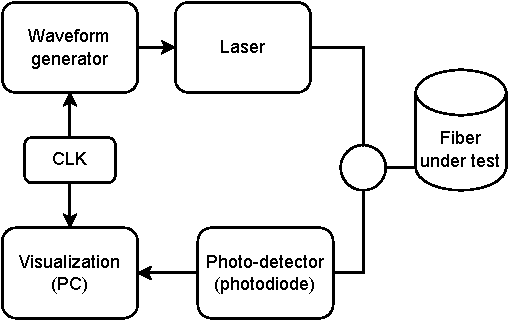
\includegraphics{pdf/optic_reflectometer.drawio.pdf}
    \caption{Example of basic OTDR reflectometer.}
    \label{fig:simpleotdr}
\end{figure}

% The goal is to use very precise light pulses with specific wavelengths, and we also  want them to be as short as possible. Unnecessarily long pulses lower the maximum pulse frequency as shown in the relation \ref{}


% \subsection{(\acs{otdr})}   %\acl{otdr} \label{txt.reflectometry.otdr2}


% %TODO
% https://www.flukenetworks.com/expertise/learn-about/otdr

% as shown in Figure~\ref{fig:otdr.diagram}.

% \cite{otdr.advances}

% \begin{figure}
%     \centering
%     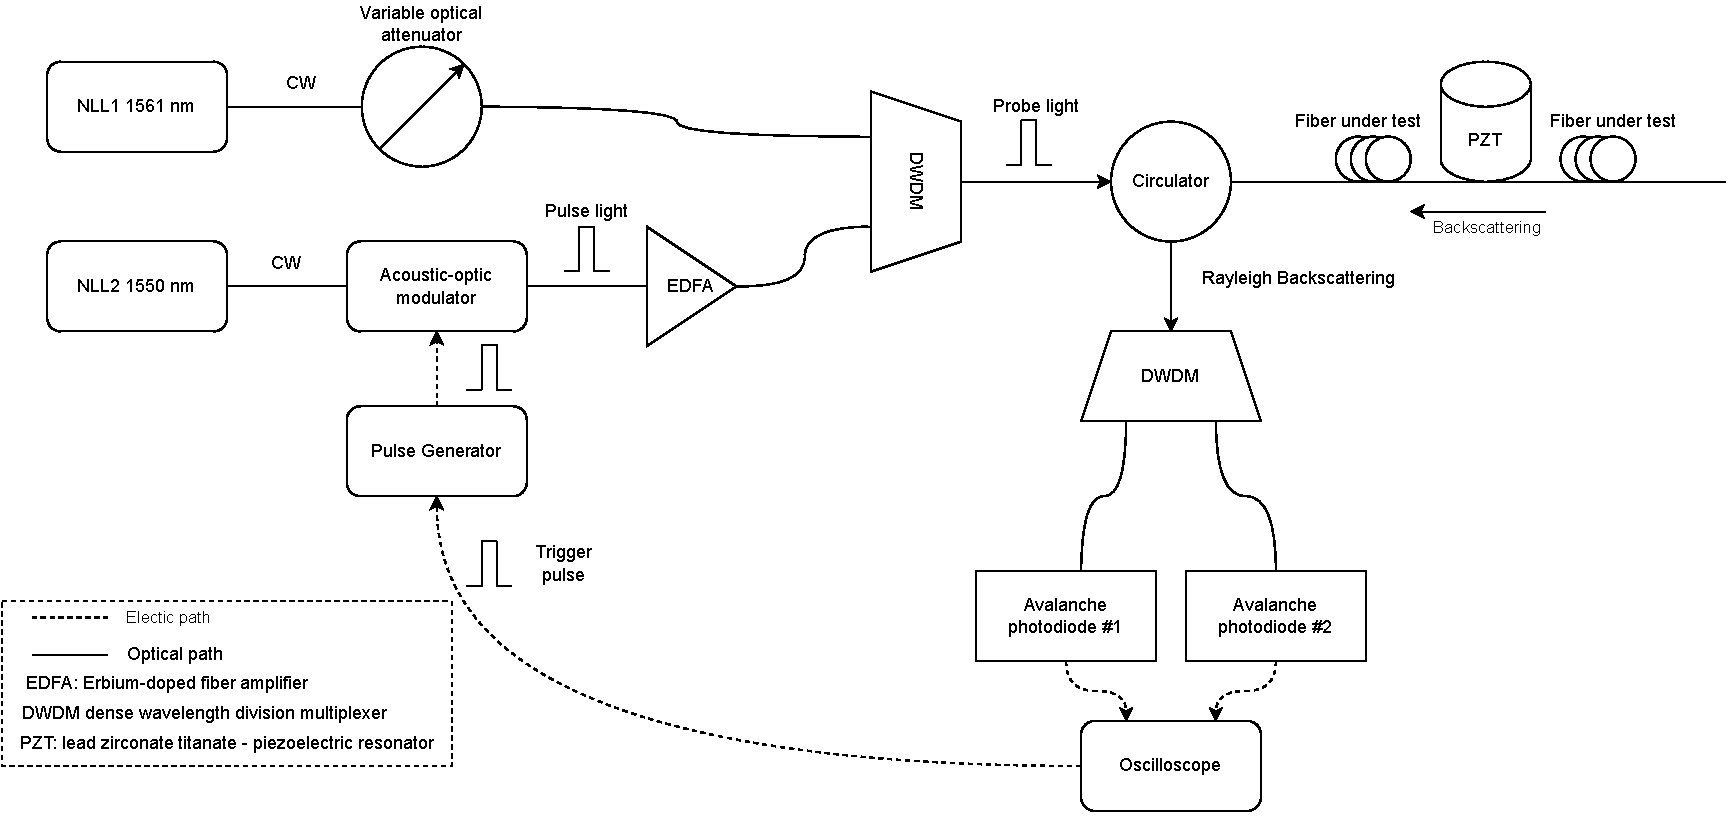
\includegraphics[width=1.5\linewidth, angle=90]{pdf/otdr.diagram.drawio.pdf}
%     \caption{Example of \ac{otdr} measuring system.}
%     \label{fig:otdr.diagram}
% \end{figure}

\subsection{OFDR}\label{txt.reflectometry.ofdr}

\ac{ofdr} analyzes interference of signal between the initial signal and the back-scattered signal but focuses on the frequency scan. A~source of light has to be a laser diode that can be precisely tuned to a certain frequency. The signal given by \ac{ofdr} contains frequency information that can be processed with the Fourier transformation. The output would be the position of the reflective elements along the fiber length. There are also other methods to measure light properties such as \textit{C-OFDR} - coherent version of OFDR using light with the frequency with linear dependency but having problems with high noise levels, and \ac{dss} - Mandelstam-Brillouin~\cite{kislov_das_newparadigm}.






























\newpage
\section{Distributed Acoustic Sensing}\label{txt.das}

Implementation of \ac{das} system is usually done by \ac{generalotdr}, \ac{ofdr}, or analysis of other light properties such as polarization and back-scatter correlation. \ac{das} allows the measurement on thousands of points on an optical wire without the need to cut the wire or have multiple sensors distributed along the wire. The measurement mechanism is based on optical reflectometry, the same as in \ac{dts}, a variant of \ac{generalotdr}. \ac{das} relies on non-uniformities spread evenly along the fiber. As discussed in Section~\ref{txt.scattering.ray}, the best suited for this application is Rayleigh scattering, which describes light scattering from particles smaller than the wavelength of the light. In this case, the particles are molecules and atoms in the fiber.

Scattering effects suitable for the use in \ac{das} measurements are Brillouin, Raman and Rayleigh 

During measurement, pulses of light are sent into the optical fiber. The fiber creates a light scattering (e.g., Rayleigh scattering) in the glass that travels back to the sensing unit (on the same side as the light source), which can be interpreted based on the arrival time as a position on the wire. Back-scattering light from the optical fiber segment is detected at the light source. If a strain or a vibration is applied to the optical fiber, it detects changes in amplitude or phase, which means that the fiber wire segment is externally affected somehow. \ac{das} is used in a wide range of applications, from locating seismic activity, locating trains along the train tracks, as a~gyroscope or an accelerometer or even as a~microphone~\cite{WangYu2017RDVM},~\cite{kislov_das_newparadigm}.

\ac{das} uses optical fiber as many sensors along its length. The fiber is capable of detecting vibrations along it can also detect acoustic properties as they are also vibrations but of sound. These sensors allow for measuring acoustic properties such as frequency, amplitude, and phase~\cite{WangYu2017RDVM}. 

When installing cables, it is crucial to consider both cable design and installation methods. The rigidity of the fiber is a significant factor because stiffer cables can reduce sensitivity. Optimal results are achieved by utilizing a single-mode fiber with minimal protection buried in the ground. The contact with the surroundings is also essential as it can impact the signal-to-noise ratio and alter the frequency content of the recorded signal.

When using an existing fiber optic infrastructure, it is hard to know what parts of the fiber are in contact with, for example, soil or ground, when measuring seismic activity, as good contact is crucial to yield good results. When monitoring boreholes, the wire can be lowered into the hole, but the quality of measurements will vary. For this purpose, mounting the cable to the bore pipe is a better solution. Good contact with the ground or seafloor is very hard to achieve, for example, in underwater applications for measuring underwater seismic activity. When laying the fiber optic cable, the cable can stretch over crevices and underwater valleys and dips, failing to make contact, which hinders the measurements and has to be accounted for.

There are also special optic fibers being developed for making the connection with the ground uniform. They have a better signal-to-noise ratio and good transmission of external vibrations on the fiber while maintaining mechanical protection~\cite{dasKislov}.

\subsection{Measurements}

The fiber is divided into segments representing a sensor located along the fiber. These sensors are just virtual - they are not real devices. By measuring time differences between the time light was transmitted and the reflected light reached the sensor, interrogator devices can identify what portion of the fiber is affected. Each segment is called \textit{Gauge Length} and represents a sensor. The location of a sensor is in the middle of the gauge length. Sometimes neighboring segments can overlap. The signal is formed between two points on the reflectogram corresponding to the edges of the gauge length. Setting gauge length is crucial to get the correct measurement. If the gauge length is too small, it degrades the signal-to-noise ratio. If too big, it creates signal distortion. Calibration is sometimes necessary to account for insufficient ground contact and to make measurements as precise as possible~\cite{dasKislov}. 

\subsection{Advantages of DAS systems}

The possibility of using existing fiber-optic infrastructure makes deploying sensing arrays very easy and cheap. Unused fiber optic wires laid for later activation, when higher bandwidth is required, are called \textit{dark-fibers} and can also be used for distributed sensing. \ac{das} technology can be applied to many different applications with the biggest advantages over the traditional sensors and electric devices in terms of no electromagnetic interference and adverse conditions - radioactivity, harsh chemical environments, high temperature, underwater, and others, see Section~\ref{txt.sensing.usage}. It is hard to imagine the limitations of this new technology~\cite{dasKislov}.

\subsection{Disadvantages to traditional sensors}

When using \ac{das} for seismology, good contact with the ground is necessary. With insufficient contact, the \ac{das} technology can provide unsuitable values. Traditional seismometers plot data instantaneously in comparison to \ac{das} systems that plot data with time delay~\cite{dasKislov}. The size of fiber-optic sensors such as fiber-optic gyroscopes is still huge compared to \ac{mems} sensors used in today's microelectronics. \ac{mems} can be soldered to PCBs and used in a wide range of applications, but they also have weaknesses, like poorer precision and low heat resistance. 

\subsection{iDAS}\label{txt.idas}

The distributed acoustic sensor is a~new addition to distributed optical fiber sensors used in the energy industry and can be used in many applications, for example, in detecting seismic activity. iDAS (intelligent distributed acoustic sensor) is one type of DAS sensor. One of the applications of this sensor is to record an acoustic signal. To determine the signal fidelity, a certain part of the wire is subjected to a known signal, for example, a sine wave. A measurement is made, and the result is compared with the existing recording device. The result suggests that iDAS has very good signal properties. The measured signal shows that almost no measurable crosstalk is exhibited between the two sensing channels on the wire.

The maximum sampling rate can be calculated from the speed of light that travels in glass at a speed of about \qty{200000}{\km/\s}, which corresponds to approximately \qty{10}{\kHz} for \qty{10}{\km} long wire~\cite{WangYu2017RDVM}.

% 10 kHz == 10 km, 1 kHz == 100 km [doplnit vzorcek]

\begin{itemize}
    \item Acoustic bandwidth.
    \item Dynamic range - \qty{120}{\dB} as reported in~\cite{dasseismic}.
    \item Spatial resolution - about \qty{1}{\m} to \qty{10}{\m}, but up to \qty{25}{\cm} is possible.
    \item Measurement range - The fiber length can be anywhere from a few hundred meters to more than \qty{100}{\km}.
\end{itemize}


\section{OptaSense ODH-F}\label{txt.optasense}

Data used in this project are obtained from \textit{OptaSense ODH-F Distributed Acoustic Sensing Interrogator}\footnote{\url{https://www.optasense.com/technology/odhf/}}(Interrogator). This device is capable of monitoring optical fiber up to \qty{50}{\km} long (in qualitative mode). It allows for sequential monitoring of four cables at the same time. It is used for in-well flow monitoring, pipeline integrity management, and border security. 

OptaSense uses \ac{cotdr}, for further explanation see Section~\ref{txt.reflectometry.otdr}

% TODO

OptaSense comes with \textit{DxS Visualization Software} capable of analyzing and processing output data from the unit. It can show the signal spectrum in a waterfall graph and create analysis, process the signal using \ac{fft}, and extract data to \verb|.wav| format. It has the limitation that it can only run in the Windows ecosystem and is proprietary software, so scientists cannot change how they work with the data or how it is displayed.

\section{Existing technology for HDF5 data visualization}\label{txt.design.existing}

This section focuses on data processing and visualization using existing software for visualizing scientific data. First is OptaSense OS6 software which is a purpose-made solution for OptaSense devices. Next is the h5web library, written in React, which creates a web page for visualizing the content of HDF5 files.



\subsection{HDF5 file format}\label{txt.hdf5}

The data captured by the Optasense Interrogator is collected in \ac{hdf} and saved into a file with \textit{.h5} suffix. \ac{hdf} creates a model for managing and storing data. The HDF Group\footnote{\url{https://www.hdfgroup.org/}} maintains the format and its corresponding software package. Specifically, the \ac{hdf} format is used to store data, but only one of the three parts makes up the full \ac{hdf} model. Parts of the \ac{hdf} model are:

\begin{itemize}
    \item File format - files ending with .h5
    \item Data model - specifies the building blocks of the \ac{hdf} file format
    \item Software - libraries, tools, APIs
\end{itemize}

\bigskip

\ac{hdf} data model has a folder-like organization, where the folders are called \textit{groups}. This model specifies the format in which the data are stored in the form of \ac{adm}, which specifies the organization of the data and the types of data. Every \ac{hdf} file has to have a~root group \textit{``/''}. Working with groups is very similar to directories on Linux systems; see Section~\ref{dir:filestructure}. Each group can have \textit{datasets} that contain raw data, attributes, data types, and other objects. \ac{hdf} file can also specify links to other libraries and tools such as compression and filtering.

\bigskip
\ac{hdf} dataset has connections with other HDF5 objects:

\begin{itemize}
    \item \textbf{attributes} - named data object containing the name and the value
    \item \textbf{datatypes}:
    \begin{itemize}
        \item Atomic datatypes - time, string, integer, float.
        \item Composite datatypes - array, enumeration, compound, variable length.
    \end{itemize}
    \item \textbf{data} - data itself, for example, the result of measurement.
    \item \textbf{dataspace} - the shape of the data.
\end{itemize}


\begin{figure}
    \centering
    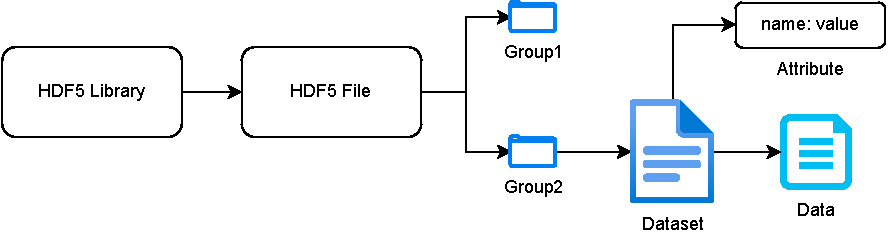
\includegraphics[width=\linewidth]{pdf/hdf5_file_structure.pdf}
    \caption{Basic HDF5 file structure.}
    \label{fig:filestructure}
\end{figure}

% \newpage


\subsection{OptaSense OS6}\label{txt.design.optasense}

The OptaSense company provides visualization software for their devices called OptaSense OS6\footnote{\url{https://www.optasense.com/technology/os/}}. It supports only Windows operating system. OS6 provides features for monitoring areas or land, for example, a compound or an industrial building. This product is tailor-made for OptaSense devices by the OptaSense company. This system has only one window for everything. The primary view is the monitored area; the background picture is the aerial view of the monitored space, as seen in the picture \ref{fig:ossix}. The user can open the sidebar on the right side. The sidebar provides multiple different options:

\begin{itemize}
    \item \textbf{Spectrogram} - Raw data visualization.
    \item \textbf{Alerts} - When an action is detected along the wire, it is logged.
    \item \textbf{Notifications} -  Notifications about system state.
    \item \textbf{System status} - Overview of all OptaSense units and their state.
\end{itemize}

There is also a feature that takes raw data from interrogator units and processes them using machine learning. This way, different actions are detected and categorized into different alerts, such as walking, driving cars, etc. In addition, the user can see the activities detected and triggered in the area overview with live monitoring and a timeline at the top of the screen. To easily look at different locations or start a new view, a feature \textit{type to search} lets the user start a search by typing into the view. For example, the user starts writing ``water...'' as a waterfall, and the program will look for this feature and open the waterfall visualization window. OS6 saves all detected activities, shown in the \textit{Historic timeline} window, which shows all alerts during a specified time range. The animations look very nice, although some look choppy, mostly when showing activities on top of the waterfall view. 

It proves that it is possible to create a real-time data visualization from the \ac{das} system. It lacks one important step, which is the ability to be used not only on Windows machines and be multi-platform. And although it provides enough tools for data analysis, it is unsuitable for further scientific work such as custom editing the visualization or exporting data to images and further processing for machine learning and activity categorization.

\begin{figure}[t]
    \centering
    \includegraphics[width=\linewidth]{obrazky/OSsix.png}
    \caption{OptaSense OS6 visualization software~\cite{ytossix}.}
    \label{fig:ossix}
\end{figure}


\subsection{h5web}\label{txt.design.h5web}

The \verb|h5web|\footnote{\url{https://h5web.panosc.eu/}} library is a set of components written in React\footnote{React is a JavaScript library used to create interactive user interface \url{https://reactjs.org/}}. H5web uses existing HDF5 libraries, such as h5wasm (reading HDF5 files in the browser) and h5grove (server for accessing HDF5 files). It displays the contents of the HDF5 file and shows different graphs according to the input from the user. From the presentation of the library by its developer, it is safe to say that although it provides the necessary equipment for opening HDF5 files elegantly and provides advanced graphing techniques, it lacks the ability to receive the data and display them as they were coming from the \ac{das} system. For this purpose, the library would need to add support by creating a new React component capable of such behavior.

\begin{figure}
    \centering
    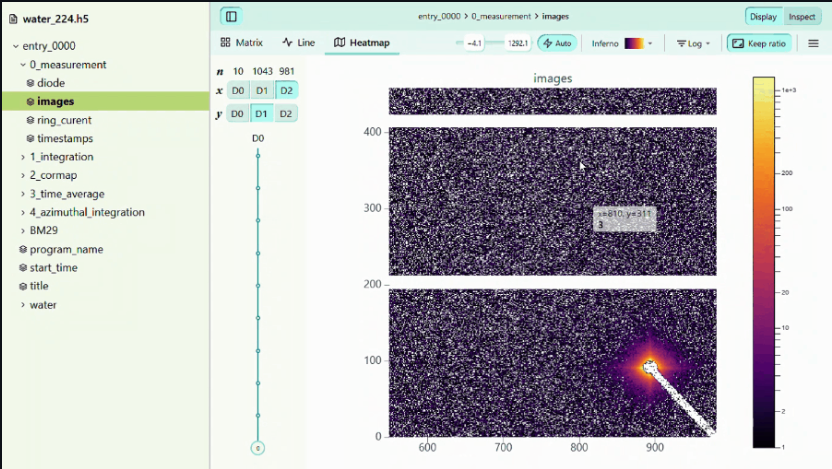
\includegraphics[width=\linewidth]{obrazky/h5web.png}
    \caption{h5web application with an example data visualization.}
    \label{fig:h5web}
\end{figure}

\newpage